\section{Auxiliary Experiments}
\label{phase_aux}

This section contains experiments and plots that were not sufficiently important, neither central to the focus of the thesis, or were otherwise \textit{auxiliary} to experiments in Sections \ref{phase1} - \ref{phase3}, but were still related and warranted being included.

\subsection{Partial Hamming Distance Measure}

From the experiments in phase~2, it became clear that for large data sets, which need speedup the most, a faster \gls{verification step} would make a considerable difference.

As discussed in Section \ref{unknown_b}, the \gls{search step} already performs some matching, and keeps track of \glspl{error}. After searching, \glspl{candidate} need to be verified to check if their overlaps' \textit{blind} components do not contain too many errors. A modification to the implementation was made to store information from the search step about the \textit{matched} component of the overlap (namely, its exact length and the counted errors within). With this knowledge, the verification step need only check the \gls{error distance} between blind components of overlaps, conceptually performing only a \textit{partial}~\gls{Hamming distance} calculation. Figure \ref{fig:partial_hamming} demonstrates the runtimes compared with and without this modification. As can be seen, the effects are consistently beneficial, but unfortunately negligible (runtime is only reduced by~2.27\% for 20,000x coverage). This is due to the fact that most of the time, the blind component is the majority of the overlap length anyway, and so the distance calculation remains largely the same. The extra space required to support this modification (2~extra numeric fields per \gls{candidate} structure) is not worth the meager speedup. As such, this modification was unfortunately rolled back.


\begin{figure}[!htb]
\centering
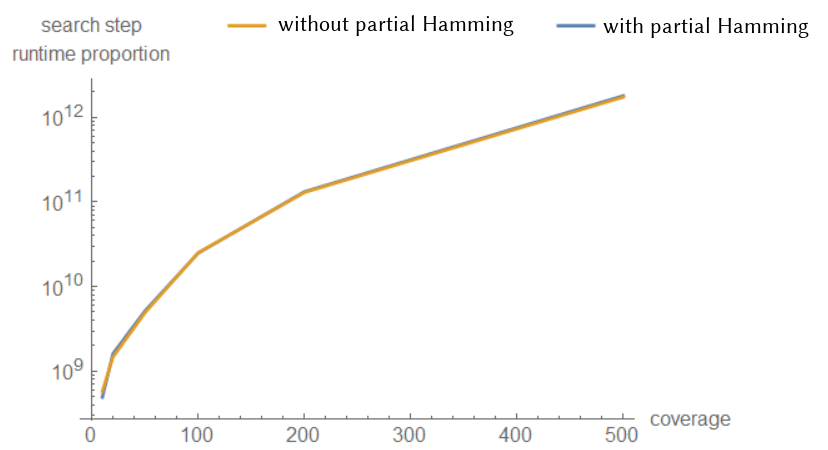
\includegraphics[width=.8\textwidth]{images/partial_hamming.png}
\caption{Comparative runtimes for executions with and without the `partial Hamming' modification across various values of coverage.}
\label{fig:partial_hamming}
\end{figure}

\subsection{Algorithm Extension Comparative Runtimes}
\label{extension_runtimes}

The \aspop{} implementation was built with the extensions from Section \ref{extensions} incorporated, enabled through the use of optional flags from the user. These extensions enrich the \gls{solution} set with new kinds of overlaps. The combination of several flags also yields unique solutions that cannot be found any other way. Of the three extensions (\gls{edit distance}, \glspl{reversal} and \glspl{inclusion}), use of reversals is most commonly advantageous for genome assembly. As such, it was used for tests throughout this work, but this need not be the case for the user.

Edit distance and inclusions are also not on by default; Although they are desirable in some cases, they are often not strictly necessary for sequence assembly, often avoided in part because they have a significant impact on runtime. Genome \gls{coverage} is shown to be a primary influence on runtime. As such, Figure \ref{fig:extensions} (a) shows the response of runtime to the use of the optional extensions, for otherwise the same problem instance; Although this figure seems to suggest that the enabling of edit distance simply scales up runtime by a constant factor, Figure \ref{fig:extensions} (b) shows that this is not the case. Using \textit{edit distance} fundamentally alters the ratios of work between the \gls{search step} and \gls{verification step} per run. Figure \ref{fig:cov} in Section \ref{phase2} would have us expect that (for edit distance disabled), the proportion of total runtime in Figure \ref{fig:extensions} (b) would fall below 50\% beyond the circa 500x \gls{coverage} mark. Unfortunately, with edit distance enabled, the runtime of this solver scales up considerably (as can be seen from (a)), forcing us to limit the coverage for this experiment to a maximum of 200x. We cannot extrapolate whether the edit-distance-enabled executions would experience runtimes with this same ratio of work in \gls{filter algorithm} steps as those of executions with edit distance disabled; Judging from the difference in behavior only within the 10x to 200x range, we would expect that the edit distance runs would likely not exhibit the `overtaking' behavior at 500x coverage seen in Figure \ref{fig:cov}.

\begin{figure}[!htb]
\centering
\makebox[\linewidth][c]{%
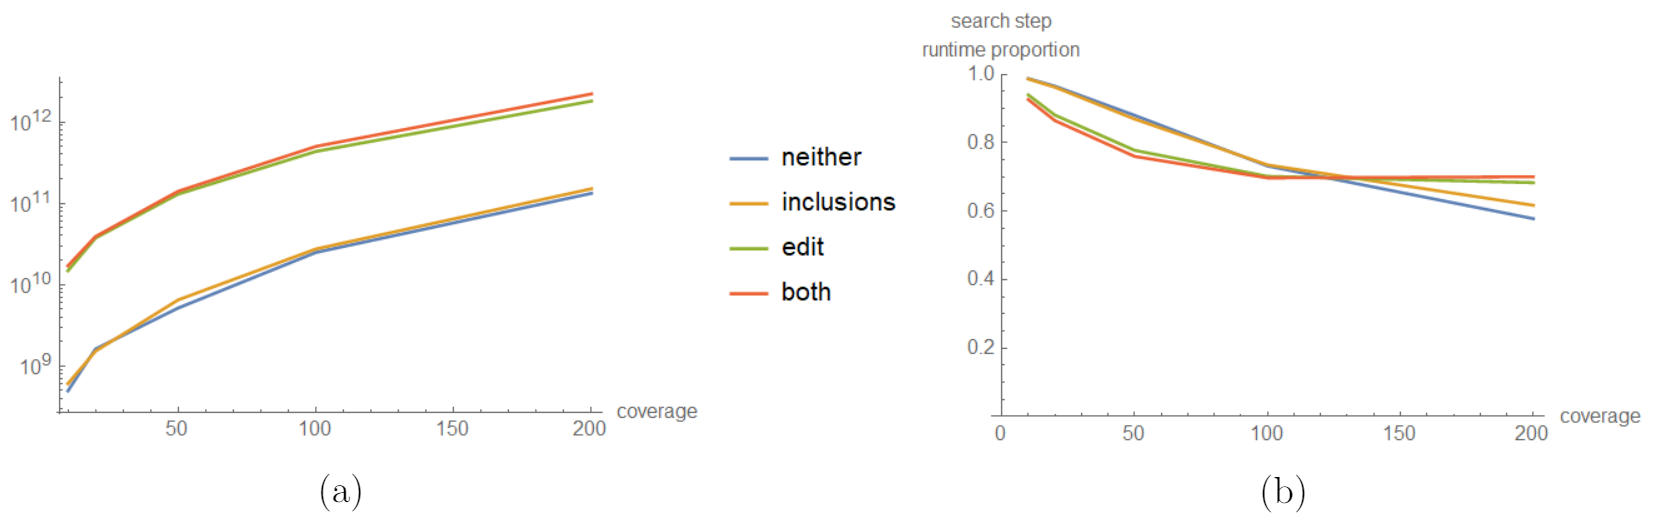
\includegraphics[width=1.15\textwidth]{images/extensions.png}
}
\caption[Runtime and runtime proportion of runs in response to coverage, with all combinations of optional flags enabling \textit{inclusions} and \textit{edit distance}.]{Runs in response to coverage, with all combinations of optional flags enabling \textit{inclusions} and \textit{edit distance} measured in terms of (a) Total runtime (b) Search step proportion of total runtime.}
\label{fig:extensions}
\end{figure}


\subsection{Runtime using \vali{}'s and Kucherov's Schemes}

Kucherov's \gls{suffix filter} algorithm introduced a new $S$ parameter (Explained in Section \ref{schemes:kuch}). In a nutshell, the choice of $S$ determines the number of \textit{redundant blocks} in the \gls{filter} associated with each search \gls{query} during the \gls{search step}. The trade-offs evident from choosing some $S$ over another yield an optimization problem, the nature of which is not immediately intuitive. 

Figure \ref{fig:schemes} demonstrates the runtime of executions using a modest viral-mix data set under the same parameters given by phase~1 in Section \ref{phase1}, in response to changing data set \gls{coverage}. \vali{}'s second algorithm resulted in significantly worse performance than Kucherov's with $S\leq{}2$ in all cases. This is consistent with Kucherov's own findings, as the \glspl{filter} in his scheme are more effective under these circumstances Additionally, Kucherov's algorithm makes use of a consistently-superior \gls{partitioning scheme}. The Kucherov run with $S=1$ behaves as the other Kucherov runs for extremely small data sets, but soon experiences \textit{extreme} slowdown in the higher-coverage run shown in Figure \ref{fig:schemes500}, much worse than that of the run using \vali{}'s second algorithm. This is a direct result of the \textit{short last block} problem explained in Section \ref{schemes:vali1} - \ref{schemes:kuch}. With $S=1$, no redundant blocks are given to the filters, resulting in the regrettable generation of hordes of \textit{spurious} \glspl{candidate}, as there are 0 completed blocks required by the \gls{candidate condition} in the \gls{query} search tree. This is especially evident in the shorter filters due to low $S$ values un-balancing the workload between filters. For this shorter run, \vali{}'s second algorithm still suffers  from its simple \gls{partitioning scheme}, relying on the work of more filters than would be necessary using Kucherov's partitioning scheme.

From all experiments conducted in this work, we observed a consistently superior runtime from Kucherov's algorithm with $S=2$. For this reason, $S=2$ is the value used elsewhere in the experiments. From Kucherov's own work, however, this trend might not continue to other problem instances with different properties beyond the bounds of our experiments \cite{kuch2014}.

\begin{figure}[!htb]
\centering
\makebox[\linewidth][c]{%
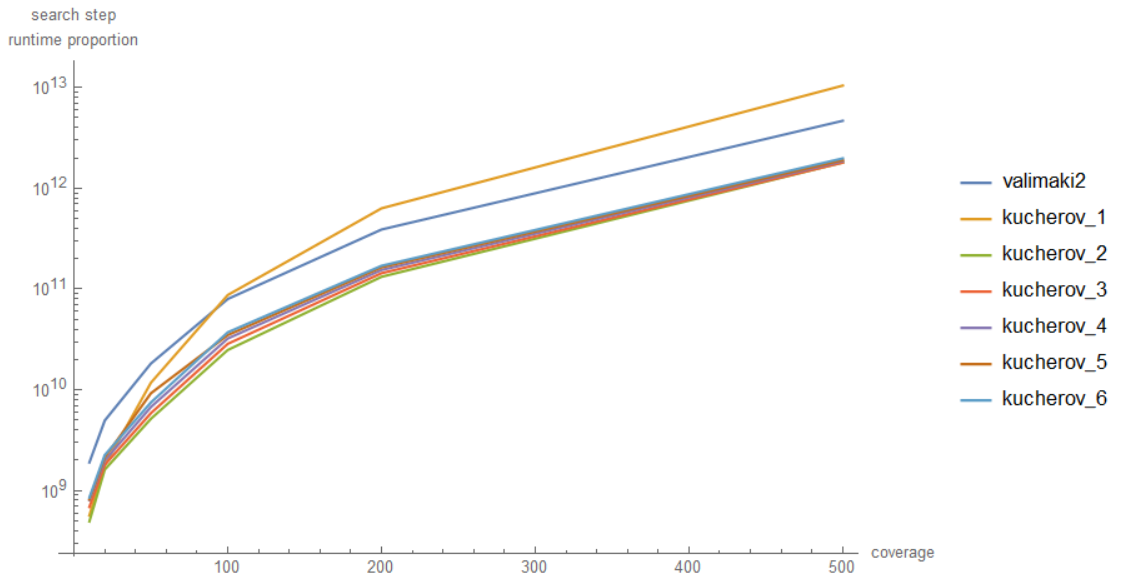
\includegraphics[width=1.0\textwidth]{images/schemes.png}
}
\caption{Comparative runtimes between \vali{}'s schemes, and Kucherov's schemes (using various values for parameter $S$), plotted in response to datasets with various values of coverage.}
\label{fig:schemes}
\end{figure}



\begin{figure}[!htb]
\centering
\makebox[\linewidth][c]{%
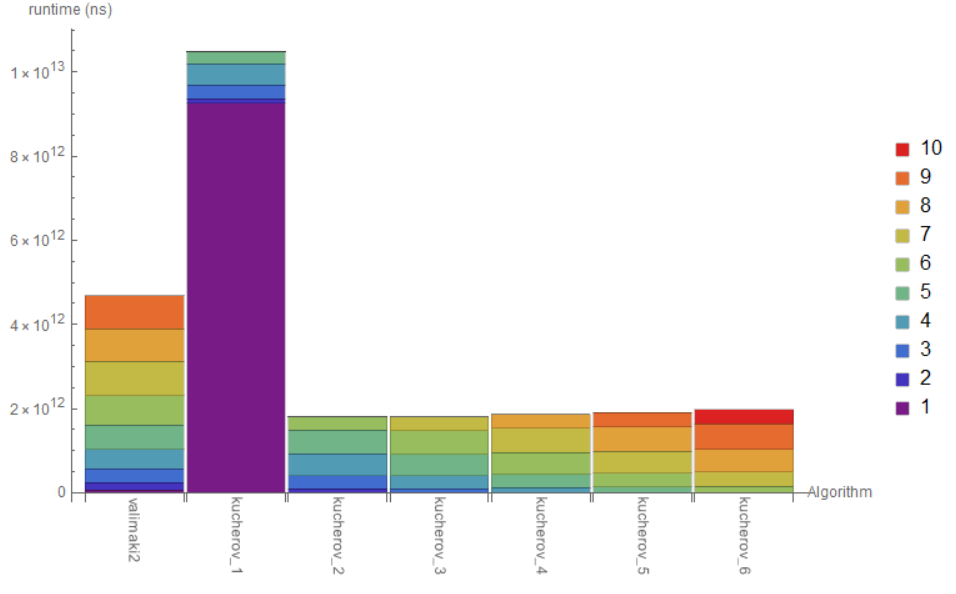
\includegraphics[width=0.9\textwidth]{images/schemes500.png}
}
\caption{Runtimes of filtering schemes of \vali{} and Kucherov, partitioned according to time per filter length, based on run `dataset\_coverage\_500x'.}
\label{fig:schemes500}
\end{figure}

\begin{figure}[!htb]
\centering
\makebox[\linewidth][c]{%
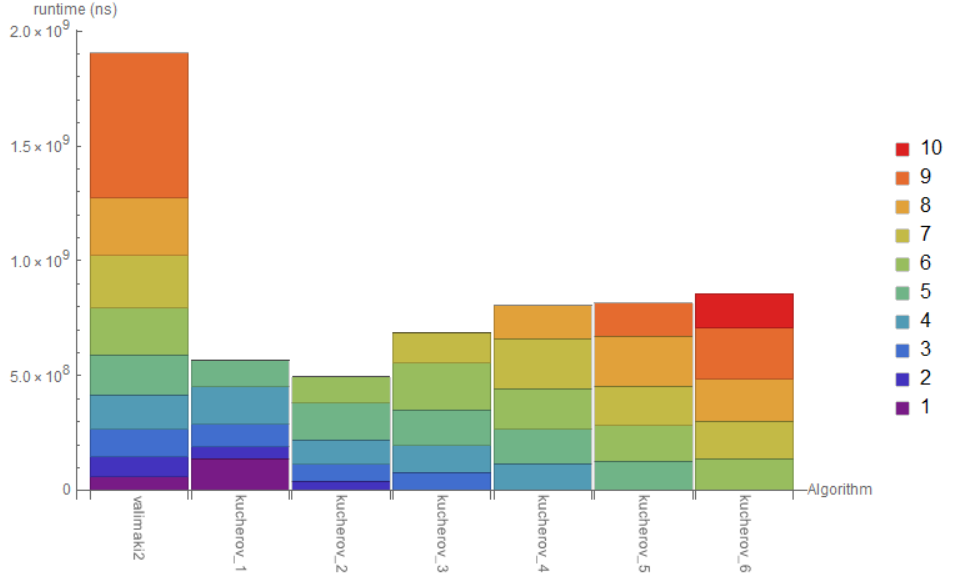
\includegraphics[width=0.9\textwidth]{images/schemes10.png}
}
\caption{Runtimes of filtering schemes of \vali{} and Kucherov, partitioned according to time per filter length, based on run `dataset\_coverage\_10x'.}
\label{fig:schemes10}
\end{figure}


\FloatBarrier
\subsection{Runtime on Full MHC Region of the Human Genome}
\label{fullmhc}

A final test of our program's speed tested its ability to handle larger data sets than were used for the numerous smaller tests. The the MHC region is located on chromosome 6, positions 28,477,797 - 33,448,354 (4,970,557 base pairs).

The run was under the same conditions as in phase 3 of the experiments, on a 24-core computer given 10 threads. After just under 25 hours, the program terminated with 1,051,648 solutions.

Unfortunately, the larger data sets showcased the differences in complexity classes between the solver. Compared to the second test in the phase 3 experiment, this data set came from a \gls{source genome} sequence 125x larger, and the run took 89,874 seconds up from 78. The run therefore took 1184x longer. By comparison, \textsc{blast} took 27 minutes to finish the same job, putting our \aspop{} solver to shame. Meanwhile, Minimap took just 34 seconds, now utterly blowing the competition out of the water in terms of speed.


\subsection{Prevalence of Pruned Nodes in Query Searches}
\label{aux:nodes}

This experiment intended to understand the practical difference between the worst-case and the typical case of the size of the \gls{query} search tree from the \gls{search step} of the \gls{suffix filter} algorithm. This section is somewhat meant as a \textit{foil} to the theoretical time complexity upper-bound defined in Section \ref{time_complexity}.

The implementation was temporarily modified to suppress pruning of \gls{query} search nodes that correspond with empty \gls{match location} sets. Instead, such nodes and all of their children are marked as `pruned' but otherwise retained. Counts of such nodes were printed to file, and the proportion computed for all searches in an execution in aggregate. It was immediately apparent during testing that the act of disabling pruning makes the solver significantly slower than before. Even the most trivial of data sets (40 \glspl{read} of 250bp) that usually takes less than a second to run didn't finish its execution in reasonable time. Thus, this experiment was run on a toy data set of generated reads with symbols sampled from a uniform distribution.

Table \ref{tab:nodes} shows the total prunable nodes in proportion to total nodes, using various combinations over ranges of \gls{read} length and number of input reads. No nodes are pruned for the 60-80 read length runs, as the search does not progress further than the first \gls{block} (with \bfit{t} set to 50). In runs with read length of 100 and beyond, an overwhelming proportion of the search tree is pruned. Naturally, the more massive search trees for longer read lengths produce more nodes; However, it becomes abundantly clear that as the search tree gets deeper, so too does the proportion of prunable nodes become even more overwhelming. In our experiment, the use of 5 significant figures was not sufficient to prevent this proportion from being indistinguishable from `1' for the largest read lengths. Although the number of reads indeed decreased the proportion of nodes pruned as expected (due to simply more \gls{text index} query hits), the proportion was modest, even between data sets with a 9-fold difference in number of reads.

As expected, the worst-case time complexity (which assumes only text index hits) is extremely pessimistic, and a user can expect a realistic execution to be \textit{lightening fast} by comparison.

\begin{table}
\centering
\caption[Proportion of nodes in query search trees pruned using Kucherov algorithm]{Proportion of nodes in query search trees pruned using Kucherov's algorithm on random data sets with $\bfit{e}=1.2\%$,  $S=2$, $\bfit{t}=50$ and reversals enabled. Read lengths (columns) ranged from 60 to 180; Number of input reads ranged from 10 to 90 (rows).\strut}
\begin{tabular}{|l||lllllll|}

\hline
 & 60 & 80 & 100 & 120 & 140 & 160 & 180 \\
\hline
\hline
10 & 0.0000 & 0.0000 & 0.9871 & 0.9909 & 0.9931 & 0.9945 & 1.0000 \\
30 & 0.0000 & 0.0000 & 0.9869 & 0.9908 & 0.9931 & 0.9945 & 1.0000 \\
90 & 0.0000 & 0.0000 & 0.9869 & 0.9908 & 0.9931 & 0.9945 & 1.0000 \\
\hline

\end{tabular}
\label{tab:nodes}
\end{table}